\documentclass{beamer}

\usepackage{epsfig,graphicx,parskip,setspace,tabularx,xspace,url,holtexbasic,alltt,proof,tikz}
\usetikzlibrary{arrows}
\usetikzlibrary{positioning}
\usetheme{CambridgeUS}

\title[Verified register allocation]{Developing a formally verified algorithm for register allocation}
\subtitle{A Part III project}
\author{David Barker}
\date{9\textsuperscript{th} June 2014}
\subject{Computer Science}


\begin{document}

\frame{\titlepage}

\section{Introduction}

\begin{frame}
\frametitle{The problem of register allocation}

\begin{itemize}
	\item Intermediate code assumes infinite registers
	\item Real machines have finite registers
	\item Using memory costs many cycles
\end{itemize}
\end{frame}

\subsection{Register allocation by graph colouring}
\begin{frame}
\frametitle{Computing live ranges}
\end{frame}

\begin{frame}
\frametitle{Building a clash graph}
\end{frame}

\begin{frame}
\frametitle{Colouring the clash graph}
\end{frame}

\begin{frame}
\frametitle{Applying the colouring}
\end{frame}

\begin{frame}
\frametitle{The full algorithm}

\begin{columns}[c]
\column{.5\textwidth}
 \begin{center}
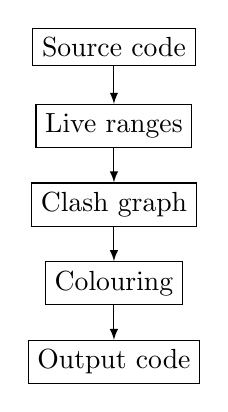
\begin{tikzpicture}[node distance = 1cm, auto]
    % Place nodes
    \node [draw] (source) {Source code};
    \node [draw, below of=source] (live) {Live ranges};
    \node [draw, below of=live] (graph) {Clash graph};
    \node [draw, below of=graph] (colouring) {Colouring};
    \node [draw, below of=colouring] (code) {Output code};
    % Draw edges
    \draw [-latex] (source) -- (live);
    \draw [-latex] (live) -- (graph);
    \draw [-latex] (graph) -- (colouring);
    \draw [-latex] (colouring) -- (code);
\end{tikzpicture}
\end{center}
\column{.5\textwidth}
 A correct algorithm will generate output code with exactly the same behaviour
\end{columns}
\end{frame}

\subsection{Guaranteeing correctness}
\begin{frame}[containsverbatim]
\frametitle{How we ensure this behaviour}
A correct algorithm produces a colouring which causes no conflicts between simultaneously live registers:

\begin{alltt}\small
	\HOLConst{colouring_ok_alt} \HOLFreeVar{c} \HOLFreeVar{code} \HOLFreeVar{live} \HOLTokenEquiv{}
\HOLConst{colouring_respects_conflicting_sets} \HOLFreeVar{c}
  (\HOLConst{conflicting_sets} \HOLFreeVar{code} \HOLFreeVar{live})
\end{alltt}

This was proved sufficient: a colouring satisfying this will always yield code with unchanged behaviour
\end{frame}

\section{Modelling the problem}
\begin{frame}[containsverbatim]
\frametitle{Code representation}
A block of code is represented by a list of three-address instructions:

\begin{alltt}\small
	\HOLTyOp{inst} = \HOLConst{Inst} \HOLKeyword{of} \HOLTyOp{num} \HOLTokenImp{} \HOLTyOp{num} \HOLTokenImp{} \HOLTyOp{num}
\end{alltt}

This is evaluated on a store $s$ as follows:

\begin{alltt}\small
	\HOLConst{eval} \HOLFreeVar{f} \HOLFreeVar{s} [] = \HOLFreeVar{s}
\HOLConst{eval} \HOLFreeVar{f} \HOLFreeVar{s} (\HOLConst{Inst} \HOLFreeVar{w} \HOLFreeVar{r\sb{\mathrm{1}}} \HOLFreeVar{r\sb{\mathrm{2}}}::\HOLFreeVar{code}) =
\HOLConst{eval} \HOLFreeVar{f} ((\HOLFreeVar{w} =+ \HOLFreeVar{f} (\HOLFreeVar{s} \HOLFreeVar{r\sb{\mathrm{1}}}) (\HOLFreeVar{s} \HOLFreeVar{r\sb{\mathrm{2}}})) \HOLFreeVar{s}) \HOLFreeVar{code}
\end{alltt}
\end{frame}

\begin{frame}[containsverbatim]
Colourings are functions of type $num \rightarrow num$

Colourings can be applied simply by substituting registers:

\begin{alltt}\small
	\HOLConst{apply} \HOLFreeVar{c} [] = []
\HOLConst{apply} \HOLFreeVar{c} (\HOLConst{Inst} \HOLFreeVar{w} \HOLFreeVar{r\sb{\mathrm{1}}} \HOLFreeVar{r\sb{\mathrm{2}}}::\HOLFreeVar{code}) =
\HOLConst{Inst} (\HOLFreeVar{c} \HOLFreeVar{w}) (\HOLFreeVar{c} \HOLFreeVar{r\sb{\mathrm{1}}}) (\HOLFreeVar{c} \HOLFreeVar{r\sb{\mathrm{2}}})::\HOLConst{apply} \HOLFreeVar{c} \HOLFreeVar{code}
\end{alltt}
\end{frame}

\begin{frame}[containsverbatim]
\frametitle{Set representation}
To simplify definitions and proofs, sets are represented as duplicate-free lists and all functions manipulating them are proven to preserve duplicate-freeness

Simple set functions:

\begin{alltt}\small
	\HOLConst{insert} \HOLFreeVar{x} \HOLFreeVar{xs} = \HOLKeyword{if} \HOLConst{MEM} \HOLFreeVar{x} \HOLFreeVar{xs} \HOLKeyword{then} \HOLFreeVar{xs} \HOLKeyword{else} \HOLFreeVar{x}::\HOLFreeVar{xs}
\end{alltt}

\begin{alltt}\small
	\HOLConst{delete} \HOLFreeVar{x} \HOLFreeVar{xs} = \HOLConst{FILTER} (\HOLTokenLambda{}\HOLBoundVar{y}. \HOLFreeVar{x} \HOLTokenNotEqual{} \HOLBoundVar{y}) \HOLFreeVar{xs}
\end{alltt}

\begin{alltt}\small
	\HOLConst{list_union} [] \HOLFreeVar{ys} = \HOLFreeVar{ys}
\HOLConst{list_union} (\HOLFreeVar{x}::\HOLFreeVar{xs}) \HOLFreeVar{ys} = \HOLConst{insert} \HOLFreeVar{x} (\HOLConst{list_union} \HOLFreeVar{xs} \HOLFreeVar{ys})
\end{alltt}

\begin{alltt}\small
	\HOLConst{list_union_flatten} [] = []
\HOLConst{list_union_flatten} (\HOLFreeVar{l}::\HOLFreeVar{ls}) =
\HOLConst{list_union} \HOLFreeVar{l} (\HOLConst{list_union_flatten} \HOLFreeVar{ls})
\end{alltt}
\end{frame}

\section{The algorithm}
\subsection{Live variable analysis}

\begin{frame}[containsverbatim]
\frametitle{Live variable analysis}
The set of live variables before a block of code is given by the following equation:

\begin{center}
$live(n) = \left(live(n+1) \setminus write(n)\right) \cup read(n)$
\end{center}

This was implemented as follows:

\begin{alltt}\small
	\HOLConst{get_live} [] \HOLFreeVar{live} = \HOLFreeVar{live}
\HOLConst{get_live} (\HOLConst{Inst} \HOLFreeVar{w} \HOLFreeVar{r\sb{\mathrm{1}}} \HOLFreeVar{r\sb{\mathrm{2}}}::\HOLFreeVar{code}) \HOLFreeVar{live} =
\HOLConst{insert} \HOLFreeVar{r\sb{\mathrm{1}}} (\HOLConst{insert} \HOLFreeVar{r\sb{\mathrm{2}}} (\HOLConst{delete} \HOLFreeVar{w} (\HOLConst{get_live} \HOLFreeVar{code} \HOLFreeVar{live})))
\end{alltt}
\end{frame}

\begin{frame}[containsverbatim]
\frametitle{Correctness}
This was implicitly proved correct as its usage led to an algorithm proven to generate behaviour-preserving colourings

More directly, it was proved that only registers returned by \texttt{get\_live} affect program behaviour:

\begin{alltt}\small
	\HOLTokenTurnstile{} (\HOLConst{MAP} \HOLFreeVar{s} (\HOLConst{get_live} \HOLFreeVar{code} \HOLFreeVar{live}) = \HOLConst{MAP} \HOLFreeVar{t} (\HOLConst{get_live} \HOLFreeVar{code} \HOLFreeVar{live})) \HOLTokenImp{}
   (\HOLConst{MAP} (\HOLConst{eval} \HOLFreeVar{f} \HOLFreeVar{s} \HOLFreeVar{code}) \HOLFreeVar{live} = \HOLConst{MAP} (\HOLConst{eval} \HOLFreeVar{f} \HOLFreeVar{t} \HOLFreeVar{code}) \HOLFreeVar{live})
\end{alltt}
\end{frame}

\subsection{Clash graph generation}
\begin{frame}
\frametitle{Clash graph representation}
Graphs are represented as lists of (vertex, clash list) pairs, for example:

$[ (r_1, [c_1, \ldots, c_n]), \ldots, (r_n, [c_1, \ldots, c_n]) ]$

Here $r_n$ is the $n^{th}$ register and $c_n$ is the $n^{th}$ register conflicting with it.

This makes it simple to iterate over vertices, and the list can be re-ordered to prioritise certain vertices for colouring.
\end{frame}

\begin{frame}[containsverbatim]
\frametitle{Building the graph}
First we need to get the list of registers conflicting with a given register:

\begin{alltt}\small
	\HOLConst{conflicts_for_register} \HOLFreeVar{r} \HOLFreeVar{code} \HOLFreeVar{live} =
\HOLConst{delete} \HOLFreeVar{r}
  (\HOLConst{list_union_flatten}
     (\HOLConst{FILTER} (\HOLTokenLambda{}\HOLBoundVar{set}. \HOLConst{MEM} \HOLFreeVar{r} \HOLBoundVar{set}) (\HOLConst{conflicting_sets} \HOLFreeVar{code} \HOLFreeVar{live})))
\end{alltt}

This function is then used to build a graph in the specified format:

\begin{alltt}\small
	\HOLConst{get_conflicts} \HOLFreeVar{code} \HOLFreeVar{live} =
\HOLConst{MAP} (\HOLTokenLambda{}\HOLBoundVar{reg}. (\HOLBoundVar{reg},\HOLConst{conflicts_for_register} \HOLBoundVar{reg} \HOLFreeVar{code} \HOLFreeVar{live}))
  (\HOLConst{get_registers} \HOLFreeVar{code} \HOLFreeVar{live})
\end{alltt}
\end{frame}

\begin{frame}[containsverbatim]
\frametitle{Correctness of generated clash graphs}
Verification of the clash graph generation stage consisted of three main proofs

The first of these states that registers never conflict with themselves, and follows easily from the definition of \texttt{conflicts\_for\_register}:

\begin{alltt}\small
	\HOLTokenTurnstile{} \HOLFreeVar{r} \HOLTokenNotIn{} \HOLConst{set} (\HOLConst{conflicts_for_register} \HOLFreeVar{r} \HOLFreeVar{code} \HOLFreeVar{live})
\end{alltt}

The second states that the graph is complete -- any registers from the same conflicting set appear in each other's conflicts:

\begin{alltt}\small
	\HOLTokenTurnstile{} \HOLConst{MEM} \HOLFreeVar{c} (\HOLConst{conflicting_sets} \HOLFreeVar{code} \HOLFreeVar{live}) \HOLTokenConj{} \HOLConst{MEM} \HOLFreeVar{r} \HOLFreeVar{c} \HOLTokenConj{} \HOLConst{MEM} \HOLFreeVar{s} \HOLFreeVar{c} \HOLTokenConj{}
   \HOLFreeVar{r} \HOLTokenNotEqual{} \HOLFreeVar{s} \HOLTokenImp{}
   \HOLConst{MEM} \HOLFreeVar{r} (\HOLConst{conflicts_for_register} \HOLFreeVar{s} \HOLFreeVar{code} \HOLFreeVar{live})
\end{alltt}
\end{frame}

\begin{frame}[containsverbatim]
Finally, it was shown that the graph doesn't contain any false conflicts -- every conflict is the result of two registers appearing in a conflicting set together:

\begin{alltt}\small
	\HOLTokenTurnstile{} \HOLConst{MEM} \HOLFreeVar{r\sb{\mathrm{1}}} (\HOLConst{conflicts_for_register} \HOLFreeVar{r\sb{\mathrm{2}}} \HOLFreeVar{code} \HOLFreeVar{live}) \HOLTokenImp{}
   \HOLTokenExists{}\HOLBoundVar{c}. \HOLConst{MEM} \HOLBoundVar{c} (\HOLConst{conflicting_sets} \HOLFreeVar{code} \HOLFreeVar{live}) \HOLTokenConj{} \HOLConst{MEM} \HOLFreeVar{r\sb{\mathrm{1}}} \HOLBoundVar{c} \HOLTokenConj{} \HOLConst{MEM} \HOLFreeVar{r\sb{\mathrm{2}}} \HOLBoundVar{c}
\end{alltt}
\end{frame}

\subsection{Colouring algorithms}

\begin{frame}[containsverbatim]
\frametitle{Defining correctness}
A graph colouring is correct if no vertex has the same colour as any of its neighbours. This is captured in the definition below:

\begin{alltt}\small
	\HOLConst{colouring_satisfactory} \HOLFreeVar{col} [] \HOLTokenEquiv{} \HOLConst{T}
\HOLConst{colouring_satisfactory} \HOLFreeVar{col} ((\HOLFreeVar{r},\HOLFreeVar{rs})::\HOLFreeVar{cs}) \HOLTokenEquiv{}
\HOLFreeVar{col} \HOLFreeVar{r} \HOLTokenNotIn{} \HOLConst{set} (\HOLConst{MAP} \HOLFreeVar{col} \HOLFreeVar{rs}) \HOLTokenConj{} \HOLConst{colouring_satisfactory} \HOLFreeVar{col} \HOLFreeVar{cs}
\end{alltt}

This was shown to imply the earlier definition of colouring correctness:

\begin{alltt}\small
	\HOLTokenTurnstile{} \HOLConst{duplicate_free} \HOLFreeVar{live} \HOLTokenImp{}
   \HOLConst{colouring_satisfactory} \HOLFreeVar{c} (\HOLConst{get_conflicts} \HOLFreeVar{code} \HOLFreeVar{live}) \HOLTokenImp{}
   \HOLConst{colouring_ok_alt} \HOLFreeVar{c} \HOLFreeVar{code} \HOLFreeVar{live}
\end{alltt}

Thus proving that a colouring satisfies \texttt{colouring\_satisfactory} is sufficient to show that it preserves program behaviour
\end{frame}

%TODO necessary?
\begin{frame}[containsverbatim]
\frametitle{Requirements on clash graphs}
For verification to work, it was necessary to show that graphs passed satisfied several properties:

\begin{itemize}
	\item Edge lists must contain no duplicates and vertices must not clash with themselves:
	
	\begin{alltt}\small
		\HOLTokenTurnstile{} \HOLConst{duplicate_free} \HOLFreeVar{live} \HOLTokenImp{}
   \HOLConst{graph_edge_lists_well_formed} (\HOLConst{get_conflicts} \HOLFreeVar{code} \HOLFreeVar{live})
	\end{alltt}
	
	\item Graphs must not contain duplicate vertices:
	
	\begin{alltt}\small
		\HOLTokenTurnstile{} \HOLConst{duplicate_free} \HOLFreeVar{live} \HOLTokenImp{}
   \HOLConst{graph_duplicate_free} (\HOLConst{get_conflicts} \HOLFreeVar{code} \HOLFreeVar{live})
	\end{alltt}
\end{itemize}
\end{frame}

\begin{frame}[containsverbatim]
\begin{itemize}
	\item Graphs must be symmetric -- if $v_1$ appears in the conflicts for $v_2$, $v_2$ appears in the conflicts for $v_1$:
	
	\begin{alltt}\small
		\HOLTokenTurnstile{} \HOLConst{duplicate_free} \HOLFreeVar{live} \HOLTokenImp{}
   \HOLConst{graph_reflects_conflicts} (\HOLConst{get_conflicts} \HOLFreeVar{code} \HOLFreeVar{live})
	\end{alltt}
\end{itemize}

These were all proven to hold of the graphs generated by the clash graph step
\end{frame}

\begin{frame}[containsverbatim]
\frametitle{Verified colouring algorithms}
The first colouring algorithm verified was a naive one which simply assigns a new colour to each vertex:

\begin{alltt}\small
	\HOLConst{naive_colouring_aux} [] \HOLFreeVar{n} = (\HOLTokenLambda{}\HOLBoundVar{x}. \HOLFreeVar{n})
\HOLConst{naive_colouring_aux} ((\HOLFreeVar{r},\HOLFreeVar{rs})::\HOLFreeVar{cs}) \HOLFreeVar{n} =
(\HOLFreeVar{r} =+ \HOLFreeVar{n}) (\HOLConst{naive_colouring_aux} \HOLFreeVar{cs} (\HOLFreeVar{n} + 1))
\end{alltt}

\begin{alltt}\small
	\HOLConst{naive_colouring} \HOLFreeVar{constraints} = \HOLConst{naive_colouring_aux} \HOLFreeVar{constraints} 0
\end{alltt}

The statement of \texttt{naive_colouring_aux}'s correctness is given below:

\begin{alltt}\small
	\HOLTokenTurnstile{} \HOLConst{graph_edge_lists_well_formed} \HOLFreeVar{cs} \HOLTokenImp{}
   \HOLTokenForall{}\HOLBoundVar{n}. \HOLConst{colouring_satisfactory} (\HOLConst{naive_colouring_aux} \HOLFreeVar{cs} \HOLBoundVar{n}) \HOLFreeVar{cs}
\end{alltt}

It was then shown that this implies the overall algorithm is correct:

\begin{alltt}\small
	\HOLTokenTurnstile{} (\HOLTokenForall{}\HOLBoundVar{n}. \HOLConst{colouring_satisfactory} (\HOLConst{naive_colouring_aux} \HOLFreeVar{cs} \HOLBoundVar{n}) \HOLFreeVar{cs}) \HOLTokenImp{}
   \HOLConst{colouring_satisfactory} (\HOLConst{naive_colouring} \HOLFreeVar{cs}) \HOLFreeVar{cs}
\end{alltt}
\end{frame}

\begin{frame}[containsverbatim]
The naive algorithm isn't at all efficient. A better algorithm is the following, which assigns to each vertex the lowest colour which won't clash with its neighbours:

\begin{alltt}\small
	\HOLConst{lowest_first_colouring} [] = (\HOLTokenLambda{}\HOLBoundVar{x}. 0)
\HOLConst{lowest_first_colouring} ((\HOLFreeVar{r},\HOLFreeVar{rs})::\HOLFreeVar{cs}) =
(\HOLKeyword{let} \HOLBoundVar{col} = \HOLConst{lowest_first_colouring} \HOLFreeVar{cs} \HOLKeyword{in}
 \HOLKeyword{let} \HOLBoundVar{lowest\HOLTokenUnderscore{}available} = \HOLConst{lowest_available_colour} \HOLBoundVar{col} \HOLFreeVar{rs}
 \HOLKeyword{in}
   (\HOLFreeVar{r} =+ \HOLBoundVar{lowest\HOLTokenUnderscore{}available}) \HOLBoundVar{col})
\end{alltt}

This was also proven correct with respect to \texttt{colouring\_satisfactory}:

\begin{alltt}\small
	\HOLTokenTurnstile{} \HOLConst{graph_reflects_conflicts} \HOLFreeVar{cs} \HOLTokenConj{} \HOLConst{graph_duplicate_free} \HOLFreeVar{cs} \HOLTokenConj{}
   \HOLConst{graph_edge_lists_well_formed} \HOLFreeVar{cs} \HOLTokenImp{}
   \HOLConst{colouring_satisfactory} (\HOLConst{lowest_first_colouring} \HOLFreeVar{cs}) \HOLFreeVar{cs}
\end{alltt}
\end{frame}


\end{document}